\documentclass[a4paper, 12pt]{article}

%%%%%%%%%%%%%%%%%%%%%%Paquetes
\usepackage[spanish]{babel}  
\usepackage{indentfirst} %%%%%%%%%%%%%%%%Crear un indent al principio
\usepackage[utf8]{inputenc}%%%%%%%%%%%%ñ y acentos
\usepackage{amstext}%%%%%%%%
\usepackage{amsfonts}%%%%%%%
\usepackage{amssymb}%%%%%%%% AMSLaTeX
\usepackage{amscd}%%%%%%%%%%
\usepackage{amsmath}%%%%%%%%
\usepackage{enumerate}%%%%%%%%%%%%%%%%Mejoras del entorno enumerate
\usepackage[all]{xy}
\usepackage{latexsym}
\usepackage{color}
\usepackage[mathcal]{eucal}%%%%%%%Caligrafica matematica
\usepackage{graphicx}
\usepackage{url}
\usepackage{tcolorbox}
\usepackage{setspace}
\onehalfspacing
%%%%%%%%%%%%%%%%%%%%%%%%%%%


%%%%%%%%%%%%%%%%%%%%%%Teoremas
\newtheorem{teo}{Teorema}[section]%%%%%%%%% Teorema
\newtheorem{defi}{Definición}[section]%%%%%%%% Definicion
\newtheorem{lema}[teo]{Lema}%%%%%%%%%%%%% Lema
\newtheorem{propo}[teo]{Proposición}%%%%%%%% Proposicion
\newtheorem{cor}[teo]{Corolario}%%%%%%%%%%%Corolario
\newtheorem{pro1}{\small Problema}%[chapter]%%%%%%%%%Problema
\newenvironment{pro}{\begin{pro1} \sf \small} {\end{pro1}}
\newtheorem{*pro1}[pro1]{* Problema}%%%%%%%%%%Problema complicado
\newenvironment{*pro}{\begin{*pro1} \sf} {\end{*pro1}}
\newcommand{\escalar}[2]{\left\langle\, #1,#2\, \right\rangle}  %%%Producto escalar 
%%%%%%%%%%%%%%%%%%%%%%%%%%%%%%%


%%%%%%%%%%%%%%%%%%%Comandos
\newcommand{\dem}{\noindent\textbf{Demostración. }\vspace{0.3 cm}}%%Demostracion
\newcommand{\R}{\mathbb{R}}%%%%%%%%%%%%Numeros reales
\newcommand{\F}{\mathbb{F}}%%%%%%%%%%%%Cuerpo
\newcommand{\C}{\mathbb{C}}%%%%%%%%%%%%Numeros complejos
\newcommand{\Q}{\mathbb{Q}}%%%%%%%%%%%%Numeros racionales
\newcommand{\N}{\mathbb{N}}%%%%%%%%%%%%Numeros naturales
\newcommand{\Z}{\mathbb{Z}}%%%%%%%%%%%%Numeros enteros
\newcommand{\g}{\mathfrak{g}}%%%%%%%%%%%%Algebra de Lie del grupo G
\newcommand{\V}{\mathcal{V}}%%%%%%%%%%%%Variedad
\newcommand{\W}{\mathcal{W}}%%%%%%%%%%%%Variedad
\newcommand{\coZ}{Z}%%%%
\newcommand{\coB}{B}%%%%  Cohomologia
\newcommand{\coH}{H}%%%%
\newcommand{\h}{\mathcal{H}}%%%%%%%%%%%%Algebra de Lie del grupo H
\newcommand{\fin}{ $\Box $ \vspace{0.4 cm}}
\newcommand{\p}{\mathfrak{p}}%%%%%%%% Ideal primo
\newcommand{\m}{\mathfrak{m}}%%%%%%%% Ideal maximal
\newcommand{\limind}{\lim_{\longrightarrow} } 
\newcommand{\gp}{\mathcal{G'}}%%%%%%%%%%%Algebra del grupo G'
\newcommand{\lto}{\longrightarrow}%%%%%%Simplificacion de la flecha larga
\newcommand{\wa}{\omega_2} %%%%%%%%%%%forma simplectica
\newcommand{\Wa}{\Omega_2} %%%%%%%%%% forma simplectica lineal
\newcommand{\lag}{\lambda_g}%%%%%%%%%%%%Traslacion a la izquierda
\newcommand{\rg}{\rho_g}%%%%%%%%%%%%%%%%Traslacion a la derecha
\newcommand{\Gr}{\boldsymbol{G}}%%%%%%%%%%Recubridor universal
\newcommand{\norma}[1]{\: \parallel #1 \!\parallel\! }%%%Norma de un vector
\newcommand{\abs}[1]{\left|\, #1 \right|}  %%%Valor absoluto 
\newcommand{\Pro}{\mathbb{P}}%%%%%%Espacio proyectivo
\newcommand{\Problemas}{\newpage  \begin{center}{\Huge Problemas}\end{center}}
\newcommand{\Ejemplos}{\vspace{0.5 cm} {\bf Ejemplos}}
\newcommand{\cpt}{\textit{cpt}}  %%%%%Casi por todo
\newcommand{\campos}{\mathfrak{X} } %%%% Campos en una variedad
\newcommand{\kulkarni}{\odot}
\renewcommand{\to}{\lto}
%%%%%%%%%%%%%%%%%%%%%%%%%%%


%%%%%%%%%%%%%%%%Operadores
\DeclareMathOperator{\End}{End}%%%%%%%%%%Endomorfismo
\DeclareMathOperator{\Ad}{Ad}%%%%%%%%%%Adjunta
\DeclareMathOperator{\grad}{grad}%%%%%%%%%%Graciente
\DeclareMathOperator{\Dif}{Dif}%%%%%%%%%%Diferenciales
\DeclareMathOperator{\sop}{sop}%%%%%%%%%Soporte
\DeclareMathOperator{\distancia}{d}%%%%%%%%Distancia
\DeclareMathOperator{\sen}{sen}%%%%%%%%%%Seno español
\DeclareMathOperator{\Der}{Der}%%%%%%%%%%Derivaciones
\DeclareMathOperator{\rang}{rang}%%%%%%%%Rango
\DeclareMathOperator{\Hom}{Hom}%%%%%%Homomorfismos
\DeclareMathOperator{\Ann}{Ann}%%%%%%%Anulador
\DeclareMathOperator{\Img}{Im} %%%%Parte imaginaria
\DeclareMathOperator{\rad}{rad}%%%%%%%%Radical
\DeclareMathOperator{\Ker}{Ker}%%%%%%%Nucleo
\DeclareMathOperator{\Id}{Id}%%%%%%% Identidad
\DeclareMathOperator{\GL}{GL}%%%%%%%%%Grupo lineal
\DeclareMathOperator{\Apli}{Apli}%%%%%%Aplicaciones
\DeclareMathOperator{\Bil}{Bil}%%%%%Bilineales
\DeclareMathOperator{\Spec}{Spec}%%%%Espectro
\DeclareMathOperator{\Ob}{Ob}  %%% Objetos de una categoría
\DeclareMathOperator{\Tor}{Tor}%%%%%Torsion de una conexión lineal
%%%%%%%%%%%%%%%%%%%%%%%%%%%%%%%


%%%%%%%%%%%%%%%%%
\title{Hipótesis de Poincaré}
\author{José Luis Tábara}
\date{jltabara@gmail.com}
%%%%%%%%%%%%%%%%%

\begin{document}



\begin{tcolorbox}[colback=red!5!white,colframe=red!75!black]

\vspace{-1cm}
\maketitle

\end{tcolorbox}

\thispagestyle{empty}

\tableofcontents

\newpage

\section*{Introducción}\setcounter{page}{1}
\addcontentsline{toc}{section}{Introducción}

 El problema fundamental de la topología es el de la clasificación: dar criterios necesarios y suficientes para que dos espacios sean homeomorfos. Dos espacios topológicos  homeomorfos son, bajo el punto de vista topológico, exactamente iguales.   El programa así descrito es enormemente ambicioso y totalmente intratable, al menos en el momento actual. Aunque no tenemos propiedades  ni invariantes adecuados para saber si dos espacios son homeomorfos, al menos tenemos bastantes criterios para afirmar  que dos espacios no pueden equivalentes. Por ejemplo, si un espacio es compacto, no puede ser homeomorfo a otro espacio que no lo sea, debido a que la compacidad es una propiedad que se conserva por aplicaciones continuas. Lo mismo se puede decir de prácticamente todos los conceptos que se estudian en la rama de las matemáticas conocida como  Topología General.  

Como la clasificación completa de los espacios topológicos es inviable, debemos restringirnos a una clase más ``selecta'' de espacios: estudiaremos únicamente las variedades topológicas de dimensión finita. Estos espacios se pueden construir ``pegando'' abiertos de un espacio euclídeo.  Si los abiertos considerados son de dimensión $n$, decimos que la variedad es de dimensión~$n$.  En algunas variedades puede ser necesario recurrir a infinitos abiertos o a abiertos con ``volumen'' infinito. Pero incluso la clasificación completa de las variedades no parece posible que sea realizada en la actualidad.  Debemos imponer algún criterio que implique de alguna manera la finitud.  Lo más natural es considerar las variedades compactas. Estas se obtienen pegando un número finito de abiertos, cada uno de los cuales tiene un volumen finito. Además se puede suponer que las variedades son conexas, puesto que las componentes conexas de cualquier variedad se pueden estudiar por separado.  Proponemos entonces el siguiente problema:

\begin{quote} \it

Clasificar todas las variedades compactas y conexas de dimensión finita

\end{quote}

El caso de la dimensión cero es trivial.  La única variedad es el punto.  El caso unidimensional también es sencillo: toda variedad conexa y compacta de dimensión 1 es homeomorfa al círculo.  Las cosas empiezan a ponerse interesantes en dimensión~2.  Este problema es equivalente al  estudio de las superficies finitas sin bordes.  En el siglo {\sc xix} se obtuvo la clasificación completa.

\smallskip

{\bf Teorema.} \begin{it}
Toda superficie compacta tiene un número natural asociado, llamado {\sf género}.  Dos superficies son homeomorfas si y solo si tienen el mismo género.
\end{it}

\smallskip

La superficie más sencilla es la esfera, que tiene género cero.  El toro tiene género 1 y la figura

\begin{figure}[htbp]
	\centering
		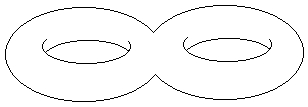
\includegraphics[width=0.70\textwidth]{imagenes/genero2.jpg}

	\label{fig:genero2}
\end{figure}


\noindent tiene género dos. En general una superficie de género $n$ es una figura similar pero con $n$ agujeros.  Intuitivamente el género mide el número de agujeros que presenta la superficie.  

\smallskip

La clasificación completa de las variedades tridimensionales se conoce como ``programa de Thurston''.  Todo el programa de clasificación, que posteriormente comentaremos,  se apoya en una piedra angular, que es la {\it conjetura de Poincaré}.  Expresada en un lenguaje vulgar dice:

\begin{quote} \it 

Si una variedad tridimensional es ``sencilla'' entonces es (equivalente) a la  esfera $S^3$

\end{quote}

\newpage

\section*{Homología}
\addcontentsline{toc}{section}{Homología}

Anteriormente hemos hablado de variedad ``sencilla''.    ¿Pero que entendemos por sencilla?  Para situarnos haremos una analogía con el caso bidimensional.  Una variedad sencilla será para nosotros una variedad sin agujeros.  Debemos estudiar entonces una teoría que de alguna manera sea capaz de estudiar los agujeros $n$-dimensionales.  Esa fué la idea de Poincaré.  La generalización que se le ocurrió a Poincaré fue la teoría de la homología. 
La idea que subyace en la teoría de la homología es el estudio de las subvariedades y sus fronteras.  Por ejemplo, en dimensión 2, si trazamos un círculo arbitrario sobre una esfera y realizamos un corte a lo largo de dicho círculo, la variedad se divide en dos partes disconexas.  El círculo es justamente el borde de cada una de las componentes conexas.  Sin embargo en un toro existen círculos tales que al cortar a traves de ellos la variedad no se desconecta.  En el toro existen círculos que no son la frontera de ninguna variedad.

\begin{figure}[htbp]
	\centering
		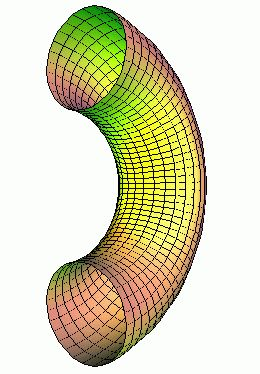
\includegraphics[width=0.40\textwidth]{imagenes/torocortado.jpg}
	\end{figure}


   En una serie de trabajos presentados a partir de 1895  Poincaré da inicio a la rama de las matemáticas conocida como Topología Algebraica. Para poder realizar cálculos, Poincaré estudia únicamente los poliedros. Define el concepto de homología de los ``poliedros'' en cualquier dimensión.  También estudia la homología de las superficies.  Para ello triangula la superficie y la deforma para convertirla en un poliedro. Las conclusiones que obtiene son independientes de la triangulación tomada y  dependen únicamente de la superficie.  Ese mismo procedimiento de triangulación puede realizarse en dimensiones superiores.   Con ello es capaz de estudiar la homología de la esfera tridimensional, que el consideraba que era la variedad tridimensional más sencilla.  Ello le lleva a formular, en 1900, una conjetura.

\begin{quote} \it

Si una variedad tridimensional tiene la misma homología que la esfera $S^3$ entonces es homeomorfa a  dicha esfera.

\end{quote}

Durante cuatro años creyó Poincaré que su conjetura era correcta, pero en 1904 encontró un contraejemplo. Construyó la variedad $\mathrm{SO}(3)/\mathrm{I}_{60}$ (donde $I_{60}$ es el grupo de isometrías de un icosaedro) cuya homología era igual a la de la esfera y sin embargo demostró que no eran homeomorfas.  Para la demostración de este hecho introdujo conceptos nuevos.  El principal era la homotopía de caminos, que es otra forma de estudiar los agujeros en dimensiones superiores.


\newpage

\section*{Homotopía}
\addcontentsline{toc}{section}{Homotopía}

Un {\it camino} en una variedad es una aplicación continua de un intervalo cerrado, pongamos $[0,1]$, en la variedad. Si denotamos por $c$ al camino, decimos que $c(0)$ es el origen del camino y que $c(1)$ es el final. 

\begin{figure}[htbp]
	\centering
		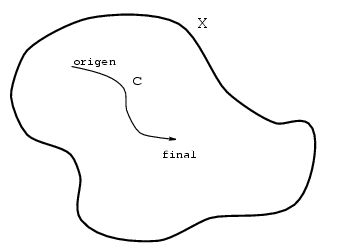
\includegraphics[width=0.45\textwidth]{imagenes/camino.jpg}

	\label{fig:camino}
\end{figure}


 En el caso particular de que el origen coincida con el final decimos que es un {\it camino cerrado} o {\it lazo}.  Consideremos ahora el conjunto de todos los lazos cuyo origen y final es un punto $p$ de la variedad.  Dados dos lazos, se puede hablar de su composición: recorremos primeramente uno y después recorremos el otro.  De esta manera obtenemos una aplicación del intervalo $[0,2]$ en la variedad.  Si hacemos que la {\it velocidad} a la que se recorren los caminos sea el doble, obtenemos un lazo definido en el intervalo unidad.  De este modo se define una operación interna en el conjunto de lazos con origen y final en~$p$.  Dado un camino $c$, llamamos inverso de $c$ al camino recorrido en sentido contrario.  La aplicación constante del intervalo unitario en $p$ se denomina camino neutro. 


 Estas definiciones pueden inducir a error, pues el conjunto de lazos con este producto no es un grupo.  Para conseguir introducir una estructura de grupo en este conjunto debemos definir una relación de equivalencia: decimos que dos caminos son equivalentes u homotópicos si se pueden deformar de manera continua uno en el otro. 
 
 
\begin{figure}[htbp]
	\centering
		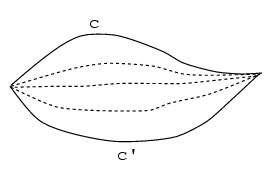
\includegraphics[width=0.45\textwidth]{imagenes/homotopiacaminosconextremos.jpg}
	\label{fig:homotopiacaminosconextremos}
\end{figure}

  El conjunto de clases de equivalencia de lazos con la composición de caminos inducida es ya un grupo.  Lo denominamos {\it grupo fundamental} o grupo de Poincaré de la variedad.  Si tomamos otro punto y la variedad es conexa por arcos (las variedades conexas lo son) el grupo obtenido es isomorfo.  En definitiva, el grupo fundamental no depende del punto base que hemos utilizado en la construcción. Además es sencillo demostrar que dos variedades homeomorfas tienen grupos fundamentales isomorfos.   Precisamente Poincaré demostró que $S^3$ y $\mathrm{SO}(3)/\mathrm{I}_{60}$ no podían ser equivalentes dado que el grupo de la esfera tenía un único elemento y el de la otra variedad tenía 120 elementos.
 
  El caso más simple es aquel en que el grupo es trivial.  Decimos que una variedad es {\it simplemente conexa} si su grupo fundamental es trivial. Ello equivale a afirmar que todo lazo se contrae a un punto. Resulta que en dos dimensiones, la esfera es la única variedad simplemente conexa.  En la figura 
\begin{figure}[h]
	\centering
		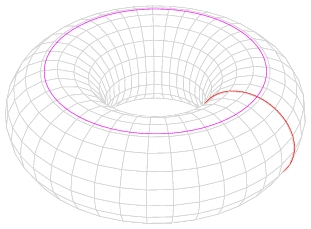
\includegraphics[width=0.50\textwidth]{imagenes/toro.jpg}
	\label{fig:toro}
\end{figure}
se observan dos lazos en un toro que no se pueden deformar a punto. Ejemplos análogos se tienen en otras superficies de género superior.  En cierto sentido, un grupo de  homotopía no trivial implica la existen de agujeros.

Hemos introducido los conceptos necesarios para formular, en términos modernos, la conjetura de Poincaré.

\begin{quote} \it

Si una variedad tridimensional tiene un grupo fundamental trivial entonces es homeomorfa a una esfera.

\end{quote}

Esta reflexión la hizo Poincaré y  añadió ``{\it mais cette question nous entraînerait trop loin'' (``pero este tema nos llevaría demasiado lejos}''). Naturalmente Poincaré no se podía imaginar que pasarían casi cien años hasta obtener la demostración.

\newpage

\section*{Dimensiones  superiores}
\addcontentsline{toc}{section}{Dimensiones superiores}


Aunque Poincaré formuló su conjetura para las variedades de dimensión 3, el mismo problema se puede plantear para cualquier dimensión. Pero ya en dimensión 4 tenemos la variedad $S^2\! \times \!S^2$, que es simplemente conexa y no es homeomorfa a la esfera $S^4$ (la homología de ambas no coincide).  Si queremos realizar un estudio análogo en dimensiones superiores debemos generalizar la afirmación de Poincaré.  La idea que subyace en la conjetura de Poincaré es que una condición relativamente debil, la homotopía, implica una condición más fuerte, que es el homeomorfismo.  Debemos clarificar que significa que dos variedades sean homotópicamente equivalentes.


\smallskip

{\bf Definición.} \begin{it}
Dadas dos variedades de la misma dimensión $X$ e $Y$, decimos que son homotópicamente equivalentes si existen aplicaciones $f: X \rightarrow Y$ y $g: Y \rightarrow X$ tales que $fg$ y $gf$ sean homotópicamente  equivalentes a la identidad.
\end{it}

\smallskip

En particular, las variedades que son  homotópicamente equivalentes a un punto se dice que son {\it contráctiles}.


La conjetura de Poincaré en dimensiónes superiores dice:

\begin{quote}\it

Si una variedad de dimensión $n$ es homotópicamente equivalente a la esfera $S^n$, entonces ambas variedades son homeomorfas.

\end{quote}

El estudio de este resultado presenta diversos problemas.  Uno de los principales es que los invariantes más destacados de las variedades, los grupos de homología y los grupos de homotopía, no son solamente invariantes por homeomorfismos, sino que también son invariantes por homotopía. Si queremos distinguir variedades que sean homotópicamente equivalentes, pero no homeomorfas, debemos introducir nuevos invariantes. A pesar de las dificultades se fue derrotando paulatinamente a la conjetura. 


En 1960 Smale demuestra la conjetura  en dimensión  igual o superior a 5. En realidad Smale no demostró la conjetura en la categoría de la variedades topológicas sino en la de variedades diferenciables, pero esos son detalles técnicos que en este momento carecen de importancia. Tan importante se consideró su trabajo que recibió por él  la medalla Fields.  Y no es el único topólogo que ha recibido tal honor por resultados directamente relacionados con la conjetura de Poincaré. 

En la misma década otros matemáticos demostraron también la conjetura de Poincaré, pero con detalles técnicos ligeramente distintos.  El principal resultado se debe a Stallings y a Zeeman que probaron la conjetura en la categoría de variedades lineales a trozos




 En 1982 Freedman demostró un resultado más general que la conjetura de Poincaré en dimensión 4. Freedman clasificó todas las variedades  simplemente conexas de dimensión 4.  Si la variedad es homotópicamente equivalente a la esfera, se obtiene como  corolario  la conjetura de Poincaré.  Otro resultado relacionado con el teorema de Freedman es la sorprendente propiedad de que $\R^4$ admite un conjunto infinito de estructuras diferenciables que no son difeomorfas.  Este caso es la excepción,  pues todos los demás espacios euclídeos tienen una estructura diferenciable única.


\newpage

\section*{Thurston y la geometría}
\addcontentsline{toc}{section}{Thurston y la geometría}


En una variedad topológica no existe ningún concepto de distancia entre puntos. Esto es ciertamente lógico, pues la métrica no se conserva por aplicaciones continuas.  Dos variedades pueden ser topológicamente equivalentes y ser sin embargo muy diferentes desde el punto de vista geométrico.  Esto no quiere decir que la geometría no sea útil a la hora de estudiar la topología. Algunas veces resultados geométricos aportan nueva luz a la topología.  Un caso especialmente importante se da en las variedades bidimensionales compactas. Ya Koebe y Poincaré demostraron  el {\it teorema de uniformización}.


\smallskip

{\bf Teorema.} \begin{it}
En toda superficie compacta (orientable) existe una métrica (de Riemann) cuya curvatura  es $0$, $1$ ó $-1$.
\end{it}

\smallskip

Este es un teorema de existencia, pero no de unicidad.  En algunas de las superficies existen en efecto varias métricas que hacen que la curvatura  sea constante.  De este modo no se puede asociar de modo canónico una única métrica a la variedad, pero si un conjunto de métricas especialmente adaptadas a dicha variedad.

 La existencia de métricas de curvatura constante reduce el problema topológico de clasificación de superficies a un problema algebraico relacionado con la teoría de grupos. 
 Para obtener todas las superficies debemos seguir varios pasos.
 
 \begin{enumerate}[\indent 1.- ]
 
 \item Primeramente debemos estudiar las variedades completas\footnote{Una variedad riemanniana es completa si cualquier geodésica se puede prolongar indefinidamente.} cuya curvatura sea $0$, $1$ ó $-1$ y que sean simplemente conexas.  En dimensión $2$ existen únicamente tres variedades de estas características: la esfera $S^2$ asociada a la curvatura $1$, el plano euclídeo $\R^2$ de curvatura nula y el plano hiperbólico $H^2$ de curvatura $-1$.
 
 
 \item Después estudiamos los grupos de isometrías de las tres variedades anteriores, comprobando que dan lugar a espacios homogéneos\footnote{Si $G$ es un grupo que actua en un espacio $X$ decimos que $X$ es un espacio homogeneo si dados dos puntos arbitrarios $x$, $x'$ existe un elemento del grupo $g$ tal que $g \cdot x = x'$}.
 
 
 \item Estudiamos los subgrupos de los grupos anteriores que cumplan que al hacer cociente por ellos se obtengan superficies compactas.  De este modo construimos todas las superficies posibles.
 
 
 \end{enumerate}
 

La idea de Thurston es la misma.  Utilizar la geometría sobre la variedad para reducir el problema de clasificación a un problema meramente algebraico, que normalmente es más sencillo. Nuestro primer problema es definir que entendemos por una geometría en tres dimensiones.

Siguiendo los pasos dados en dos dimensiones, debemos encontrar modelos de variedades tridimensionales que sean simplemente conexas, que sean completas y que sean homogeneas.  Como además estamos interesados en el caso compacto debemos ver cuales de esas geometrías dan lugar a variedades compactas al hacer cociente.  Thurston resolvió el problema (y recibió por ello una medalla Fields) y encontró que había exactamente 8 geometrías tridimensionales con cocientes compactos.  Tres de ellas son las asociadas a las curvatura constante positiva, negativa y nula. Las otras se obtienen básicamente al hacer productos y analizar métricas invariantes en grupos de Lie. Podemos dar entonces la 


\smallskip

{\bf Definición.} \begin{it}
Una {\it estructura geométrica} en una variedad es una métrica de Riemann completa y localmente homogenea (su recubridor universal es homogéneo).
\end{it}

\smallskip


Existen variedades tridimensionales que no admiten ninguna estructura geométrica, debido a obtrucciones de tipo topológico.  Thurston sabía que era posible realizar cirugía con dichas variedades y descomponerlas en varias componentes.   Para ello debía hechar mano de resultados ya conocidos.  El primero de ellos de ellos se conoce como {\it descomposición prima} y afirma que toda variedad compacta se puede cortar a lo largo de esferas bidimensionales dando lugar a varias componentes.  Cada una de estas componentes no puede ser dividida del mismo modo y por lo tanto decimos que es {\it prima}. La descomposición obtenida de este modo es única salvo homeomorfismos.  Después a cada una de las componentes primas se le puede aplicar la {\it descomposición tórica}, donde los cortes esta vez se dan a lo largo de toros. Ya podemos enunciar la {\it conjetura de Thurston}:

\begin{quote} \it

Dada una variedad tridimensional compacta, después de efectuar la descomposición prima y la descomposición tórica, cada una de las componentes admite una estructura geométrica.

\end{quote}


Se ha demostrado la validez de la conjetura en algunos tipos de variedades, pero todavía no se sabe si es o no correcta.  Los trabajos de Perelman parecen indicar que si.


Si la conjetura es cierta, el problema de clasificación de las variedades tridimensionales compactas se reduce al estudio y clasificación de las 8 geometrías.  De estas 8, 6 están perfectamente estudiadas y clasificadas.  En las otras 2 se conocen muchas cosas, pero el tema todavía no está cerrado. A proposito, las dos que peor se conocen no  son ninguna de las geometrías ``raras'' sino la esférica y la hiperbólica.


En particular, la conjetura de Poincaré, es un simple corolario de este resultado.  Si fuese  falsa, también sería falsa la conjetura de Thurston y la clasificación de las variedades tridimensionales sería más compleja de lo que creemos en este momento.

\newpage

\section*{El flujo de Ricci}
\addcontentsline{toc}{section}{El flujo de Ricci}

El problema de la existencia de métricas con características especiales sobre las variedades siempre ha cautivado a los matemáticos. Ejemplos típicos son los teorema de uniformización y el problema de Yamabe.  En el mejor de los casos, si la métrica es única, se pueden realizar cálculos con dicha métrica y obtener información topológica.  El modo habitual de atacar este problema es proponer un problema variacional en el espacio de las métricas y los extremos de ese problema es probable que sean métricas con características espaciales.

Sin embargo, en la década de los 80, Hamilton inventa un nuevo método, denominado {\it flujo de Ricci}. En realidad la idea no es nueva, pues el flujo de Ricci se estudia habitualmente en Relatividad General, pero aplicado a métricas semirriemannianas. En este caso se estudian ecuaciones diferenciales ordinarias (en dimensión infinita) que debe satisfacer la métrica. Se introduce  una métrica arbitraria en la variedad,  se hace evolucionar mediante la ecuación diferencial y se observa si converge a alguna solución.  En el conjunto de métricas de Riemann de una variedad se pueden proponer muchas ecuaciones diferenciales diferentes, pero el flujo de Ricci es la ecuación más sencilla.  Su expresión analítica es
$$
\frac{d g}{d t}=-2Ric_{g(t)} +\lambda(t) \cdot g
$$
donde $g$ denota la métrica riemanniana y $Ric$ el tensor de Ricci asociado. 
Hamilton estudió el caso en que $\lambda$ es nulo y llegó a interesantes resultados.  El principal es que si el tensor de Ricci es definido positivo en todo punto, la métrica evoluciona, tras una renomalización, hacia una métrica de curvatura constante positiva.  En una variedad donde se pueda introducir una métrica cuyo tensor de Ricci sea definido positivo la conjetura de geometrización es cierta.  

Pero al estudiar el flujo en el caso general se presentaban singularidades y no era posible demostrar la conjetura de geometrización.

 Si la métrica varía de acuerdo al flujo de Ricci, la curvatura escalar evoluciona mediante la ecuación
$$
\frac{d R}{dt}= \Delta R + 2 \sum {Ric}^{ij}_{ij}
$$
que es una ecuación similar a la del calor pero no líneal. 

\newpage

\section*{Bibliografía}
\addcontentsline{toc}{section}{Bibliografía}



\begin{itemize}\small

\item John Milnor. {\it The Poincaré Conjecture One Hundred Years Later.}

 \verb|http://www.math.sunysb.edu/~jack/|

\item Michael T. Anderson. {\it Geometrization of 3-Manifolds Via the Ricci Flow.} \verb|http://www.math.sunysb.edu/~anderson/|


\item John Milnor. {\it Towars the Poincaré Conjecture and the Classification of \mbox{3-Manifolds.}} \verb|http://www.math.sunysb.edu/~jack/|

\item Graham P. Collins. {\it Las Formas del Espacio.} Investigación y Ciencia, Octubre 2004.

\item Michael T. Anderson. {\it Scalar Curvature and Geometrization Conjectures for 3-Manifolds.}\verb|http://www.math.sunysb.edu/~anderson/|

\item Michael Kapovic. {\it Geometrization Conjecture and Ricci Flow.}

 \verb|http://www.math.ucdavis.edu/~kapovich/|



\end{itemize}



\end{document}